\captionsetup{justification=centering,margin=0cm}
\label{cap:atividade7}  % Forma de referenciar o capítulo no comando \ref

%inicio do capitulo
\chapter[Atividade7: Otimizando imagens]{Atividade 7: Otimizando imagens}
Será que já exploramos todas as formas de compressão e otimização possíveis? Giraldeli acredita que não. Por isso, vamos analisar e discutir o software PINGO e sua interface gráfica, PINGA, desenvolvida pelo próprio criador.
Na imagem abaixo, é possível observar as taxas médias de compressão, tanto em modos lossless quanto "lossy"/Near-lossless (explicaremos isso em breve), a partir de imagens PNG-24 adquiridas das imagens originais.

\begin{table}[H]
\centering
\caption{Otimização de imagens em PNG}
\begin{tabularx}{\textwidth}{X|C|C|C|C}
\hline
\multirow{2}{*}{\textbf{\makecell[c]{PNG Original\\(bytes)}}} & \multicolumn{2}{c|}{\textbf{\textit{Lossless}}} & \multicolumn{2}{c}{\textbf{\textit{Near-Lossless}}} \\ \hhline{~----}
~ & Tamanho (bytes) & Ratio (\%) & Tamanho (bytes) & Ratio (\%) \\ \hline

113.944.706 & 109.971.161 & 96,51\% & 46.038.976 & 40,40\% \\
\hline
\end{tabularx}

\autoriaPropria
\end{table}

\paragrafo De início, percebe-se que o formato lossless não oferece uma redução significativa. No entanto, o modo Near-lossless surgiu como uma solução promissora e interessante.

\paragrafo O formato Near-lossless é um método de compressão com perdas (lossy) que visa otimizar outros formatos de compressão. Nesse formato, pequenas variações pontuais que dificultariam a compressão lossless são eliminadas. Por exemplo, em uma imagem de um céu limpo, pode haver várias tonalidades de azul. O Near-lossless "padroniza" essas tonalidades (sem que haja mudanças visíveis) para que, após a aplicação de uma compressão realmente lossless, a eficiência seja muito maior.

\paragrafo A tabela a seguir apresenta dados relativos à compressão Near-lossless utilizada.

\begin{table}[H]
    \centering
    \caption{Avaliação dos Artefatos do JPEG}
    \label{tab:6b}

    \footnotesize
    \begin{tabularx}{\textwidth}{X|C|C|C}
    \hline
        Descrição & Tamanho PNG Original & Tamanho PNG Near-lossless & Redução (\%) \\ \hline
        IMG01 & 1.613.669 & 470.751 & 70,8\% \\ 
        IMG02 & 2.126.163 & 744.135 & 65,0\% \\ 
        IMG03 & 1.042.306 & 276.561 & 73,5\% \\ 
        IMG04 & 1.822.802 & 586.640 & 67,8\% \\ 
        IMG05 & 1.885.248 & 517.736 & 72,5\% \\ 
        IMG06 & 1.915.684 & 707.084 & 63,1\% \\ 
        IMG07 & 1.572.060 & 445.175 & 71,7\% \\ 
        IMG08 & 3.513.270 & 1.988.475 & 43,4\% \\ 
        IMG09 & 1.960.195 & 589.413 & 69,9\% \\ 
        IMG10 & 2.509.826 & 889.026 & 64,6\% \\ 
        IMG11 & 3.224.670 & 1.472.274 & 54,3\% \\ 
        IMG12 & 2.569.986 & 1.014.155 & 60,5\% \\ 
        IMG13 & 2.568.571 & 965.602 & 62,4\% \\ 
        IMG14 & 2.329.559 & 934.462 & 59,9\% \\ 
        IMG15 & 1.156.266 & 250.572 & 78,3\% \\ 
        IMG16 & 2.489.280 & 1.006.796 & 59,6\% \\ 
        IMG17 & 2.466.793 & 921.658 & 62,6\% \\ 
        IMG18 & 1.906.284 & 616.201 & 67,7\% \\ 
        IMG19 & 2.683.151 & 1.079.954 & 59,8\% \\ 
        IMG20 & 3.127.814 & 1.648.449 & 47,3\% \\ 
        IMG21 & 1.582.110 & 596.268 & 62,3\% \\ 
        IMG22 & 2.649.058 & 1.113.681 & 58,0\% \\ 
        IMG23 & 2.246.862 & 930.639 & 58,6\% \\ 
        IMG24 & 2.412.455 & 1.250.916 & 48,1\% \\ 
        IMG25 & 2.287.870 & 838.609 & 63,3\% \\ 
        IMG26 & 1.676.966 & 568.036 & 66,1\% \\ 
        IMG27 & 3.220.560 & 1.526.112 & 52,6\% \\ 
        IMG28 & 2.325.051 & 1.089.100 & 53,2\% \\ 
        IMG29 & 692.210 & 244.930 & 64,6\% \\ 
        IMG30 & 1.445.622 & 338.954 & 76,6\% \\ 
        IMG31 & 1.881.345 & 905.145 & 51,9\% \\ 
        IMG32 & 2.533.661 & 925.294 & 63,5\% \\ 
        IMG33 & 2.956.042 & 1.499.003 & 49,3\% \\ 
        IMG34 & 2.046.515 & 534.616 & 73,9\% \\ 
        IMG35 & 2.304.984 & 904.325 & 60,8\% \\ 
        IMG36 & 1.092.302 & 390.488 & 64,3\% \\ 
        IMG37 & 2.822.178 & 1.121.492 & 60,3\% \\ 
        IMG38 & 3.048.615 & 1.410.537 & 53,7\% \\ 
        IMG39 & 2.564.862 & 1.133.122 & 55,8\% \\ 
        IMG40 & 2.384.943 & 826.070 & 65,4\% \\ 
        IMG41 & 3.048.024 & 1.488.942 & 51,2\% \\ 
        IMG42 & 1.187.267 & 311.156 & 73,8\% \\ 
        IMG43 & 2.814.564 & 1.300.451 & 53,8\% \\ 
        IMG44 & 3.201.971 & 1.568.705 & 51,0\% \\ 
        IMG45 & 2.506.005 & 1.117.689 & 55,4\% \\ 
        IMG46 & 2.332.555 & 902.688 & 61,3\% \\ 
        IMG47 & 2.309.341 & 778.783 & 66,3\% \\ 
        IMG48 & 3.387.244 & 1.815.708 & 46,4\% \\ 
        IMG49 & 2.044.998 & 536.091 & 73,8\% \\ 
        IMG50 & 2.454.929 & 946.307 & 61,5\% \\ \hline
        \textit{MÍNIMO} & 692.210 & 244.930 & 43,4\% \\ 
        \textit{MÉDIO} & 2.278.894 & 920.780 & 61,4\% \\ 
        \textit{MÁXIMO} & 3.513.270 & 1.988.475 & 78,3\% \\ 
    \end{tabularx}

    \autoriaPropria
\end{table}

\paragrafo com estes dados, é possível observar que as melhores compressões ocorrem em imagens com poucas cores ou com grandes áreas monocromáticas, como nas imagens 1, 3, 5, 7, 15, 30, 34 e 42, onde todas apresentam mais de 70\% de redução.

\paragrafo Num geral, as imagens geradas são fascinantes\footnote{Durante as comparações das imagens, fiquei muito tempo analizando se as cores das imagens estavam diferentes ou se era loucura da minha cabeça kk}, é em sua grande maioria transparente a imagem original e é enormemente mais eficiente (em bytes), se levarmos em consideração o fato de ser "lossless".

\paragrafo Abaixo estão são demonstrados uma comparação antes e depois da compressão nas imagens 11 e 15.

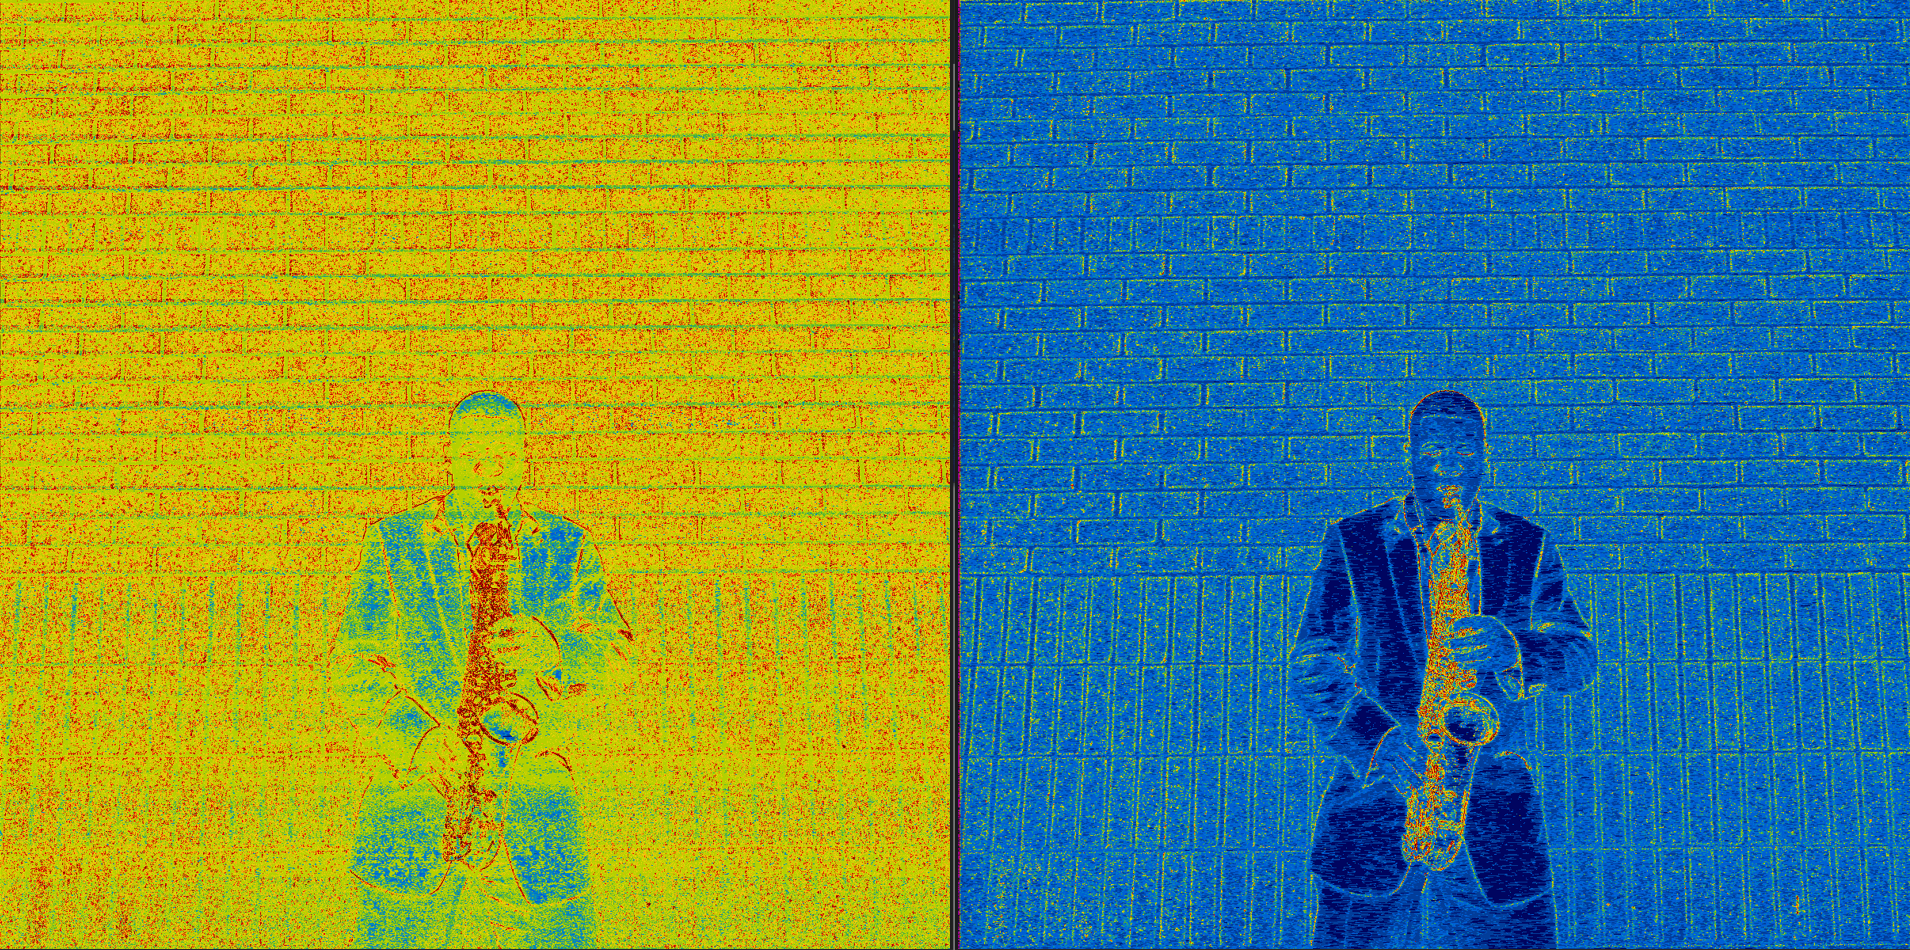
\includegraphics[scale=0.24]{Documeto/1-ElementosTextuais/1-Desenvolvimento/Imagens-atividade7/IMG11.png}

\includegraphics[scale=0.24]{Documeto/1-ElementosTextuais/1-Desenvolvimento/Imagens-atividade7/IMG15.png}

\paragrafo Vale ressaltar também a tabela de relação entre cor e quantidade de bits utilizados, imagem, retirada dos slides da matéria, abaixo:

\includegraphics[scale=0.35]{Documeto/1-ElementosTextuais/1-Desenvolvimento/Imagens-atividade7/Tabela.png}


\paragrafo Com base nas imagens, observamos que há uma redução expressiva de complexidade entre elas, resultando em um arquivo .png muito mais otimizado.\footnote{A diferença de coloração da imagem utilizando o pngthermal é bizarroooo}

\paragrafo Entretanto, como nem tudo são flores, houve exceções que, após a aplicação do método supracitado, apresentaram mudanças visíveis. Começando pelas diferenças menores:

Observamos que nas imagens 21 e 44, o céu apresentava vários pontos espalhados (apesar de ser necessário dar zoom para observá-los com clareza).
Na imagem 5, há uma mudança imperceptível sem a presença da imagem original. Na água, há ladrilhos que são mais visíveis na imagem original, enquanto na imagem com a técnica aplicada, eles ficam opacos.
Na imagem 39, há uma camada no céu.
Finalmente, as falhas mais visíveis, sendo possível observá-las facilmente, estão nas imagens 15 e 29. Ambas apresentam macroblocos visíveis. Na imagem 29, pequenos macroblocos aparecem na parte inferior direita da flor. Entretanto e Surpreendentemente, a imagem 15, que apresentou o melhor percentual de compressão, também apresentou a pior compressão em termos visuais, com macroblocos muito visíveis facilmente no canto inferior direito da imagem.

\paragrafo De modo geral, o software apresentado demonstrou ser extremamente útil e eficiente, alcançando uma taxa média de compressão (ratio) de 38,6 a partir da imagem original. Isso o torna uma opção viável para armazenar um grande volume de fotos, especialmente para fins de recordação e em situações em que a qualidade da imagem é mais importante do que a otimização.

\paragrafo Desta forma, também é interessante buscarmos melhores compressões para aqueles que priorizam maiores otimizações, mantendo a qualidade das imagens. Vamos abordar a compressão Lossy, utilizando um software que compara a imagem original com várias versões dela, cada uma com um fator Q diferente, permitindo ajustar o parâmetro de mudança média. Ficou confuso? Vou explicar melhor.

\paragrafo Abaixo, apresentamos a redução em \% das compressões realizadas, utilizando o padrão do software. A "Redução JPEG Câmera" refere-se à redução adicional feita sobre a compressão realizada pela própria câmera.

\begin{table}[H]
    \centering
    \caption{Otimizando Imagens em JPEG (Modo Lossy, em KB)}
    \label{tab:6b}

    \footnotesize
    \begin{tabularx}{\textwidth}{X|C|C|C|C|C}
    \hline
        Imagem & Tam Sem Compressão & Tam. JPEG Câmera & Ratio JPEG Câmera (\%) & Tam. JPEG Otimizado & \% Redução JPEG Câmera \\ \hline
        IMG01 & 26.791 & 2.278 & 8,5\% & 1199 & 47,4\% \\ 
        IMG02 & 26.791 & 1.777 & 6,6\% & 814 & 54,2\% \\ 
        IMG03 & 26.791 & 3.151 & 11,8\% & 1710 & 45,7\% \\ 
        IMG04 & 26.791 & 2.512 & 9,4\% & 1244 & 50,5\% \\ 
        IMG05 & 26.791 & 7.918 & 29,6\% & 718 & 90,9\% \\ 
        IMG06 & 26.791 & 1.814 & 6,8\% & 1438 & 20,7\% \\ 
        IMG07 & 26.791 & 2.113 & 7,9\% & 1009 & 52,2\% \\ 
        IMG08 & 26.791 & 3.977 & 14,8\% & 2115 & 46,8\% \\ 
        IMG09 & 26.791 & 2.312 & 8,6\% & 1578 & 31,7\% \\ 
        IMG10 & 26.791 & 2.100 & 7,8\% & 1381 & 34,2\% \\ 
        IMG11 & 26.791 & 5.724 & 21,4\% & 3373 & 41,1\% \\ 
        IMG12 & 26.791 & 2.409 & 9,0\% & 1290 & 46,5\% \\ 
        IMG13 & 26.791 & 5.227 & 19,5\% & 2966 & 43,3\% \\ 
        IMG14 & 26.791 & 2.733 & 10,2\% & 1524 & 44,2\% \\ 
        IMG15 & 26.791 & 4.460 & 16,6\% & 2745 & 38,5\% \\ 
        IMG16 & 26.791 & 3.646 & 13,6\% & 1878 & 48,5\% \\ 
        IMG17 & 26.791 & 2.386 & 8,9\% & 1353 & 43,3\% \\ 
        IMG18 & 26.791 & 1.156 & 4,3\% & 696 & 39,8\% \\ 
        IMG19 & 26.791 & 1.561 & 5,8\% & 1113 & 28,7\% \\ 
        IMG20 & 26.791 & 5.005 & 18,7\% & 2897 & 42,1\% \\ \hline
        \textbf{MÍNIMO} & 26.791 & 1.156 & 4,3\% & 696 & 20,7\% \\ 
        \textbf{MÉDIO} & 26.791 & 3.213 & 11,99\% & 1.652 & 44,5\% \\ 
        \textbf{MÁXIMO} & 26.791 & 7.918 & 29,6\% & 3.373 & 90,9\% \\ 
    \end{tabularx}

    \autoriaPropria
\end{table}

\paragrafo Pode-se observar que já alcançamos uma boa otimização, mas, surpreendentemente, o fator de qualidade está no nível mais alto, preservando o máximo de qualidade, embora menos otimizado. Observando as imagens lado a lado ou sequencialmente, todas parecem absolutamente idênticas nos testes realizados. Contudo, não paramos por aí. Decidi testar a compressão no índice mínimo de fidelidade, mesmo que isso impactasse a transparência das imagens. Os dados e imagens dos resultados serão mostrados a seguir.

\begin{table}[H]
    \centering
    \caption{Otimizando Imagens em JPEG LOW(Modo Lossy, em KB)}
    \label{tab:6b}

    \footnotesize
    \begin{tabularx}{\textwidth}{X|C|C|C|C|C}
    \hline
        Imagem & Tam Sem Compressão & Tam. JPEG Câmera & Ratio JPEG Câmera (\%) & Tam. JPEG Otimizado (low)\textbf{} & \% Redução JPEG Câmera \\ \hline 
        IMG01 & 26.791 & 2.278 & 8,5\% & 537 & 76,4\% \\ 
        IMG02 & 26.791 & 1.777 & 6,6\% & 278 & 84,4\% \\ 
        IMG03 & 26.791 & 3.151 & 11,8\% & 666 & 78,9\% \\ 
        IMG04 & 26.791 & 2.512 & 9,4\% & 476 & 81,1\% \\ 
        IMG05 & 26.791 & 7.918 & 29,6\% & 251 & 96,8\% \\ 
        IMG06 & 26.791 & 1.814 & 6,8\% & 356 & 80,4\% \\ 
        IMG07 & 26.791 & 2.113 & 7,9\% & 378 & 82,1\% \\ 
        IMG08 & 26.791 & 3.977 & 14,8\% & 732 & 81,6\% \\ 
        IMG09 & 26.791 & 2.312 & 8,6\% & 473 & 79,5\% \\ 
        IMG10 & 26.791 & 2.100 & 7,8\% & 434 & 79,3\% \\ 
        IMG11 & 26.791 & 5.724 & 21,4\% & 1344 & 76,5\% \\ 
        IMG12 & 26.791 & 2.409 & 9,0\% & 535 & 77,8\% \\ 
        IMG13 & 26.791 & 5.227 & 19,5\% & 1088 & 79,2\% \\ 
        IMG14 & 26.791 & 2.733 & 10,2\% & 584 & 78,6\% \\ 
        IMG15 & 26.791 & 4.460 & 16,6\% & 1153 & 74,1\% \\ 
        IMG16 & 26.791 & 3.646 & 13,6\% & 658 & 82,0\% \\ 
        IMG17 & 26.791 & 2.386 & 8,9\% & 556 & 76,7\% \\ 
        IMG18 & 26.791 & 1.156 & 4,3\% & 323 & 72,1\% \\ 
        IMG19 & 26.791 & 1.561 & 5,8\% & 191 & 87,8\% \\ 
        IMG20 & 26.791 & 5.005 & 18,7\% & 1050 & 79,0\% \\ \hline
        \textbf{MÍNIMO} & 26.791 & 1.156 & 4,3\% & 191 & 72,1\% \\ 
        \textbf{MÉDIO} & 26.791 & 3.213 & 11,99\% & 603 & 80,2\% \\ 
        \textbf{MÁXIMO} & 26.791 & 7.918 & 29,6\% & 1.344 & 96,8\% \\ 
    \end{tabularx}

    \autoriaPropria
\end{table}

\paragrafo Nos testes realizados com a resolução no nível mais baixo (maior otimização), nem todas as imagens mantêm a transparência perfeita. No entanto, as mudanças são mínimas, tornando viável, em nossa opinião, o uso consistente desse método. As únicas alterações perceptíveis ocorreram nas sombras das imagens 1, 2, 3, 4, 12\footnote{Durante a realização dos testes, ficávamos alternando entre as imagens em tela cheia no monitor, e na imagem 12, teve uma situação engraçada, nela parecia ter uma espécie de sobrancelha subindo e descendo conforme alternavamos entre as imagens}, 15, 16 e 17, de forma trivial. Portanto, quando se trata de otimização de imagens com foco em maior compressão, este método é extremamente eficiente.
